\documentclass{beamer}
\usetheme{Warsaw}

\usepackage[utf8]{inputenc}
\usepackage{fancybox}
\usepackage{multimedia} 
\usepackage{subfig}
\usepackage{amsmath}

\usepackage[all]{xy}
\begin{document}


\title[Computergrafik] % (optional, only for long titles)
{Computergrafik

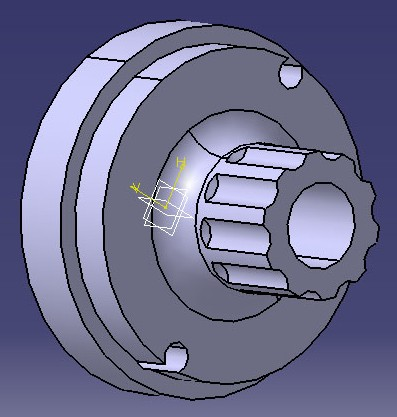
\includegraphics[scale=0.36]{images/CAD3D}
}
\subtitle{}
\author[Dr. Johannes Riesterer] % (optional, for multiple authors)
{Dr.  rer. nat. Johannes Riesterer}

\date[KPT 2004] % (optional)
{}

\subject{Computergrafik}



\begin{frame}
    \frametitle{Algorithmen und Datenstrukturen}
\framesubtitle{}
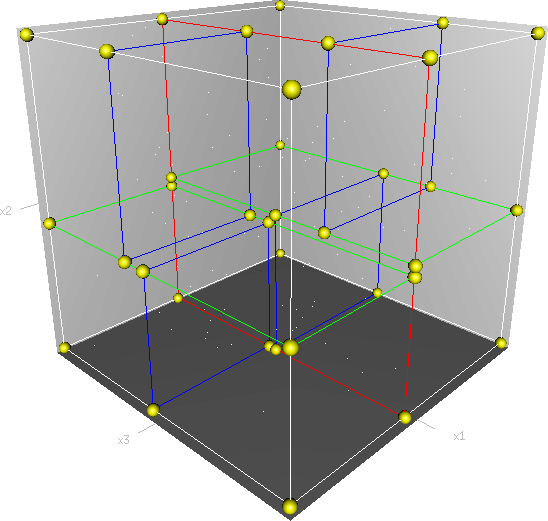
\includegraphics[scale=0.42]{images/3dtree}
\end{frame}

\begin{frame}
    \frametitle{Algorithmen und Datenstrukturen}
\framesubtitle{}
    \begin{block}{Z-Buffer}

Der Z-Buffer enthält für jedes Pixel $(u,v)$ nach der Rasterung  einen Wert zwischen $-1$ und $1$. Dieser Wert  ist der Abstand zum nächsten Punkt eines Polygons  in Clipping-Koordinaten von diesem Pixel auf der Projektionsebene.  Wir haben somit eine Funktion


\begin{align*}
Z-Buffer : \mathbb{N} \times \mathbb{N} \to [-1,1]  \; .
\end{align*}

\begin{figure}[H]
    \centering
    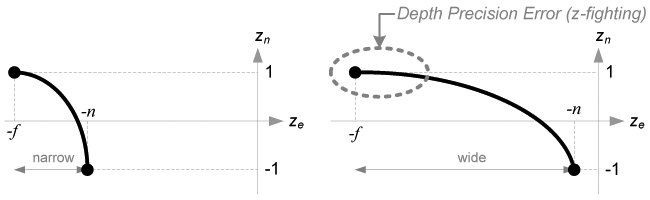
\includegraphics[width=0.9\textwidth]{images/gl_projectionmatrix_zbuffer_1.png}
    \caption{Z-Buffer-War}
    \label{fig:zbuffer-war}
\end{figure}

\end{block}

\end{frame}


\begin{frame}
    \frametitle{Algorithmen und Datenstrukturen}
\framesubtitle{}
\begin{block}{Shadowmap}
Das Rendern einer Szene mit Schatten unter Zuhilfenahme von einer Shadow Map geschieht im Wesentlichen in zwei Schritten. Als erstes wird die Szene aus der Sicht des Lichts gerendert und die Tiefeninformation (z-Buffer) in eine Textur gerendert. Anschließend wird die Szene normal gerendert, wobei für jedes Pixel  der Abstand des zugehörigen Vertex zur Lichtquelle (in Clipping Coordinaten) mit dem Wert der Shadow Map verglichen wird. Ist der Wert in der Shadow Map kleiner, wird  das Pixel schattiert gerendert.
\end{block}
\end{frame}
\begin{frame}
    \frametitle{Algorithmen und Datenstrukturen}
\framesubtitle{}
\begin{figure}[H]\centering
    \subfloat[Tiefeninformation aus Sicht des Lichtes gerendert]{
        \hspace*{0.025\textwidth}
         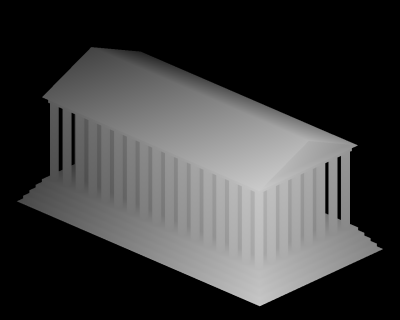
\includegraphics[width=0.35\textwidth]{images/sm_zb.png}
    \label{fig:shadowmap3}
    }
    \hspace*{0.1\textwidth}
    \subfloat[Rendering ohne Shadow mapt]{
        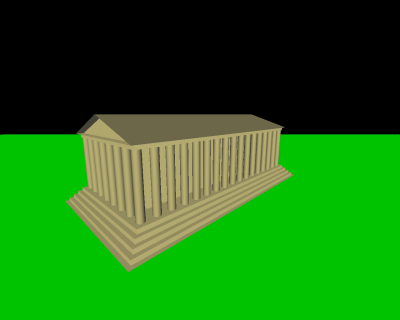
\includegraphics[width=0.35\textwidth]{images/sm_ns.png}
    \label{fig:shadowmap1}
    }
    \vspace*{1em}
    \subfloat[Rendering mit Shadow map]{
        \hspace*{0.025\textwidth}
         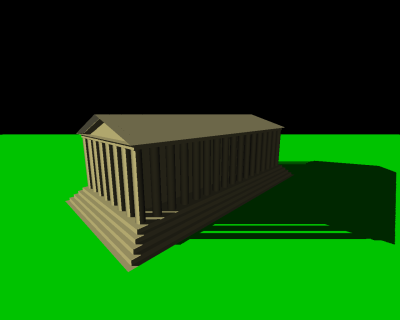
\includegraphics[width=0.35\textwidth]{images/sm_ws.png}
    \label{fig:shadowmap2}
    }
\end{figure}

\end{frame}




\begin{frame}
    \frametitle{Algorithmen und Datenstrukturen}
\framesubtitle{}
    \begin{block}{Texturemapping}
    Ein Texturemapping ist eine Abbildung $T: \mathbb{R}^2 \to \mathbb{R}^3$, 
    die Bildpunkte den Vertices des Meshes zuordnet.
    \end{block}

\begin{figure}[H]
    \centering
    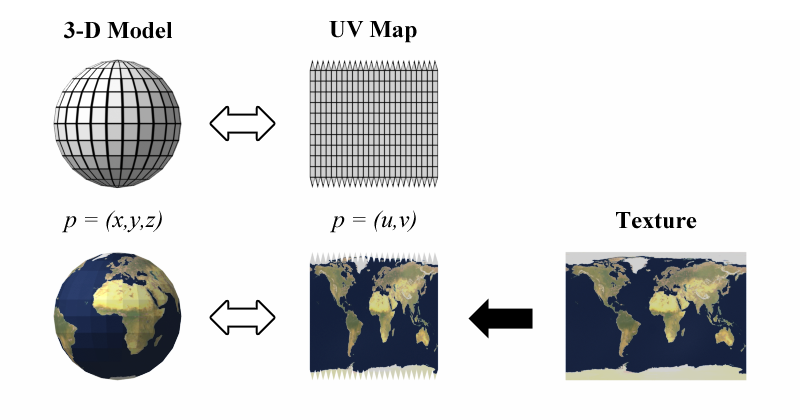
\includegraphics[width=0.75\textwidth]{images/tm_uv.png}
    \caption{uv mapping} %TODO: fix caption&label
    \label{fig:uv-mapping1}
\end{figure}
\end{frame}

\begin{frame}
    \frametitle{Algorithmen und Datenstrukturen}
\framesubtitle{}
\begin{figure}[H]
    \centering
    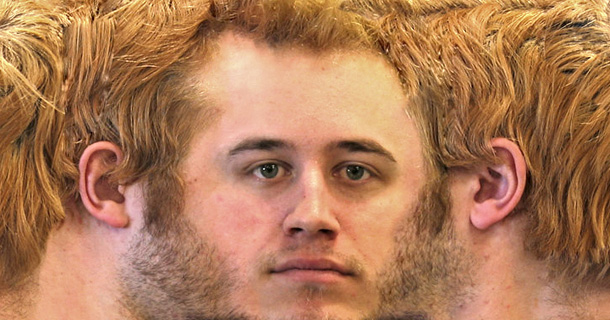
\includegraphics[width=1.0\textwidth]{images/tm_face.jpg}
    \caption{uv mapping} %TODO: fix caption&label
    \label{fig:uv-mapping2}
\end{figure}
\end{frame}



\begin{frame}
    \frametitle{Algorithmen und Datenstrukturen}
\framesubtitle{}
    \begin{block}{Bumpmapping}

        Die relativen Höheninformationen liegen in einer Textur (Hightmap) in Form von Graustufen vor – der sogenannten Heightmap. 
        Jeder Grauwert steht für eine bestimmte Höhe. 
        Für die Lichtberechnung werden Normalen berechnet, 
        die einem Netz entprechen,
        welches entsteht, wenn man die Vertices entlang der ursprünglichen Normale um den Betrag in der Bumpmap verschiebt.  
        
        \begin{figure}[H]
            \centering
            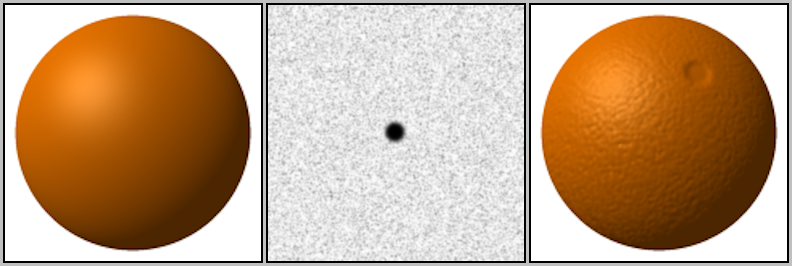
\includegraphics[width=0.9\textwidth]{images/Bumpmap.png}
            \caption{Bumpmapping} %TODO: fix caption&label
        \end{figure}
        
\end{block}

\end{frame}


\begin{frame}
    \frametitle{Algorithmen und Datenstrukturen}
\framesubtitle{}
    \begin{block}{Bumpmapping}


Wie beim Bumpmapping  wird  eine Heightmap als Textur mitgegeben.
Im Gegensatz dazu werden die Punkte des Gitternetzes (Vertices)  entsprechend diesen Texturinformationen entlang ihrer Normalen, 
das heißt senkrecht zur Oberfläche, tatsächlich verschoben. 

\begin{figure}[H]
    \centering
    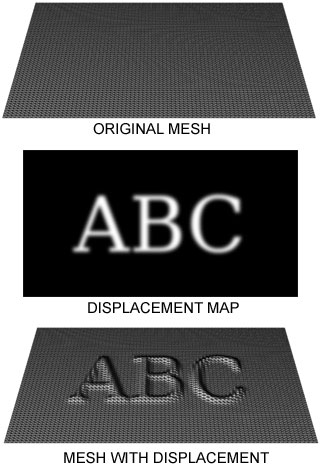
\includegraphics[width=0.25\textwidth]{images/Displacement.jpg}
    \caption{Displacementmapping} %TODO: fix caption&label
    \label{fig:displacement-mapping}
\end{figure}

\begin{figure}[H]
    \centering
    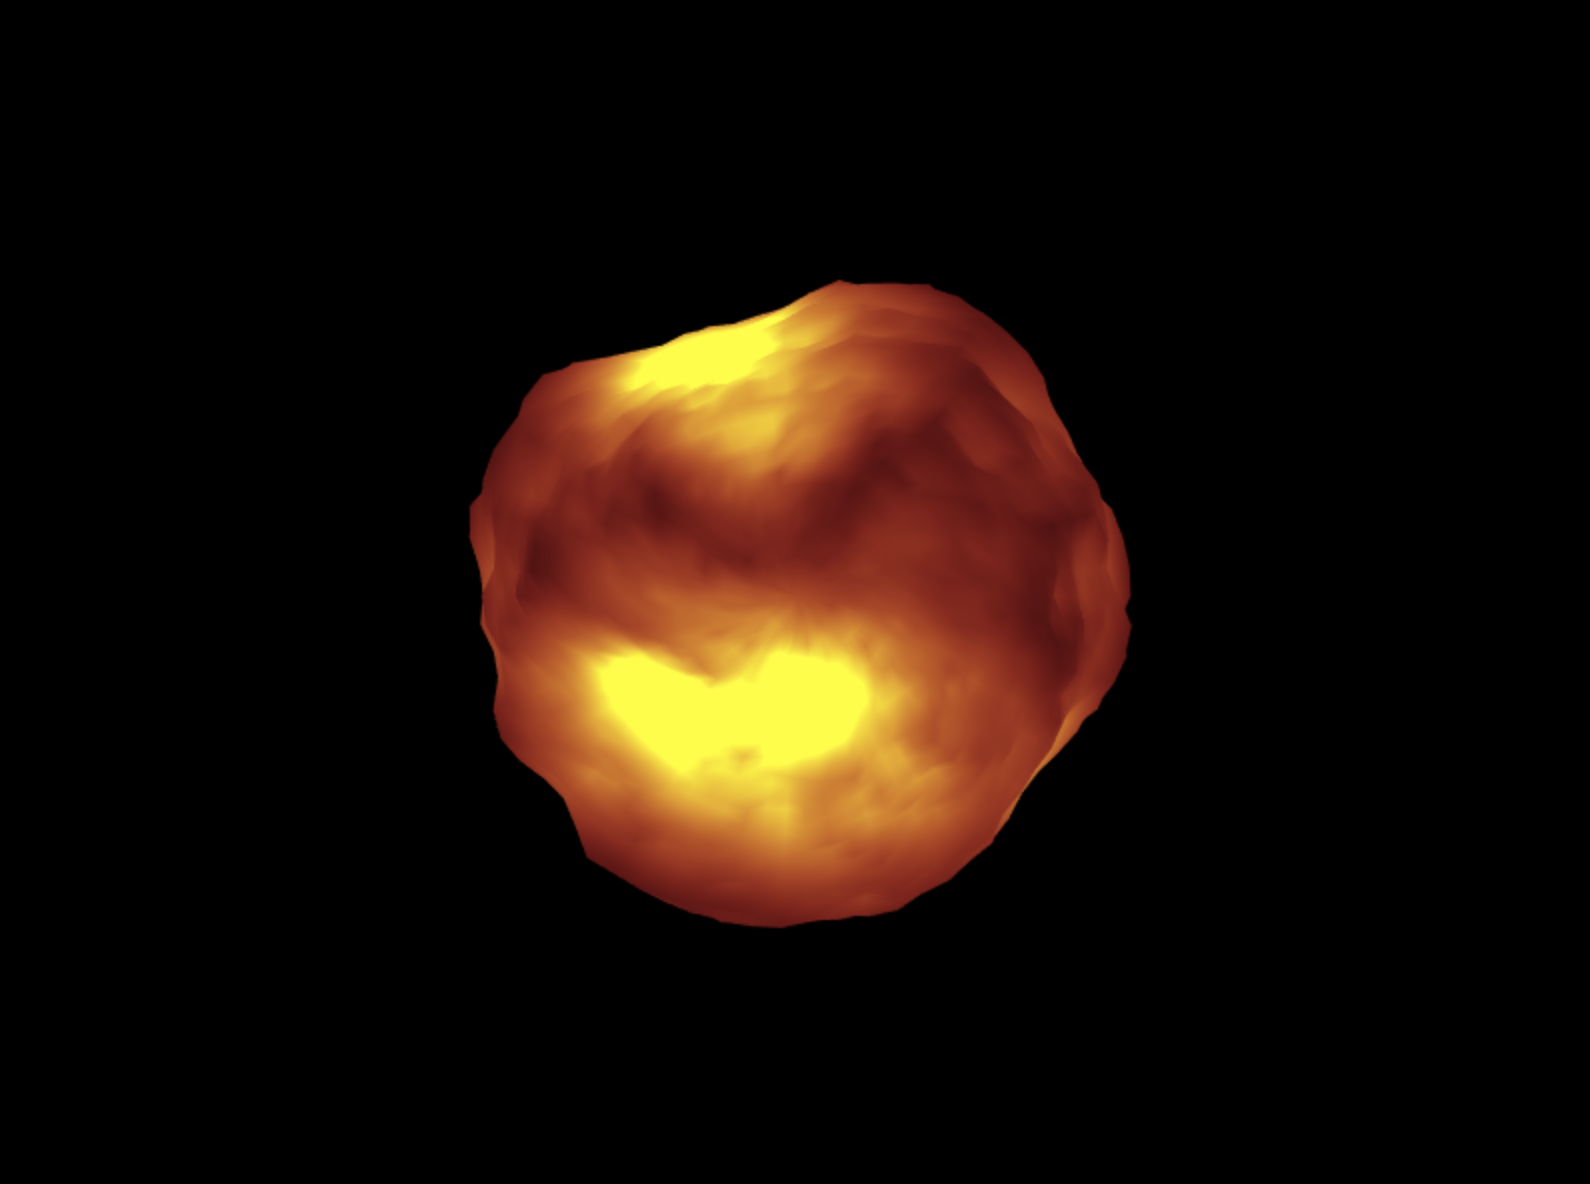
\includegraphics[width=0.4\textwidth]{images/lava.png}
    \caption{Lavaball}
    \label{fig:reflection-phong-specular-model}
\end{figure}
\end{block}

\end{frame}


\begin{frame}
    \frametitle{Algorithmen und Datenstrukturen}
\framesubtitle{}
\begin{block}{Perlin Noise}
Perlin Noise ist ein Algorithmus zur Erzeugung zufälliger, 
organischer Strukturen. 
Die Entwicklung geht auf Ken Perlin zurück, 
der ihn 1982 für den Film Tron entwickelte, 
wofür er 1997 einen Oscar erhielt
\end{block}
\end{frame}


\begin{frame}
    \frametitle{Algorithmen und Datenstrukturen}
\framesubtitle{}
\begin{figure}[H]
    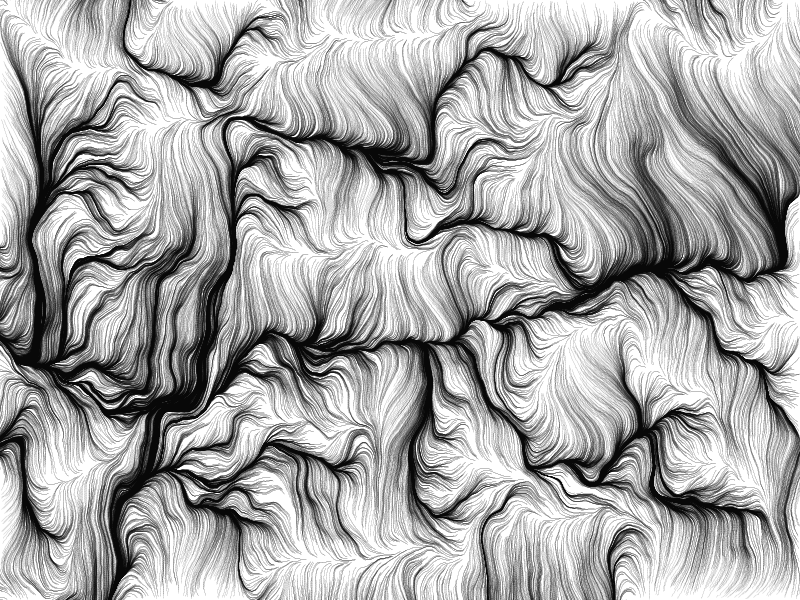
\includegraphics[width=0.4\textwidth]{images/perlinnoisepattern.png}
    \caption{Anwenung Perlin Noise}
    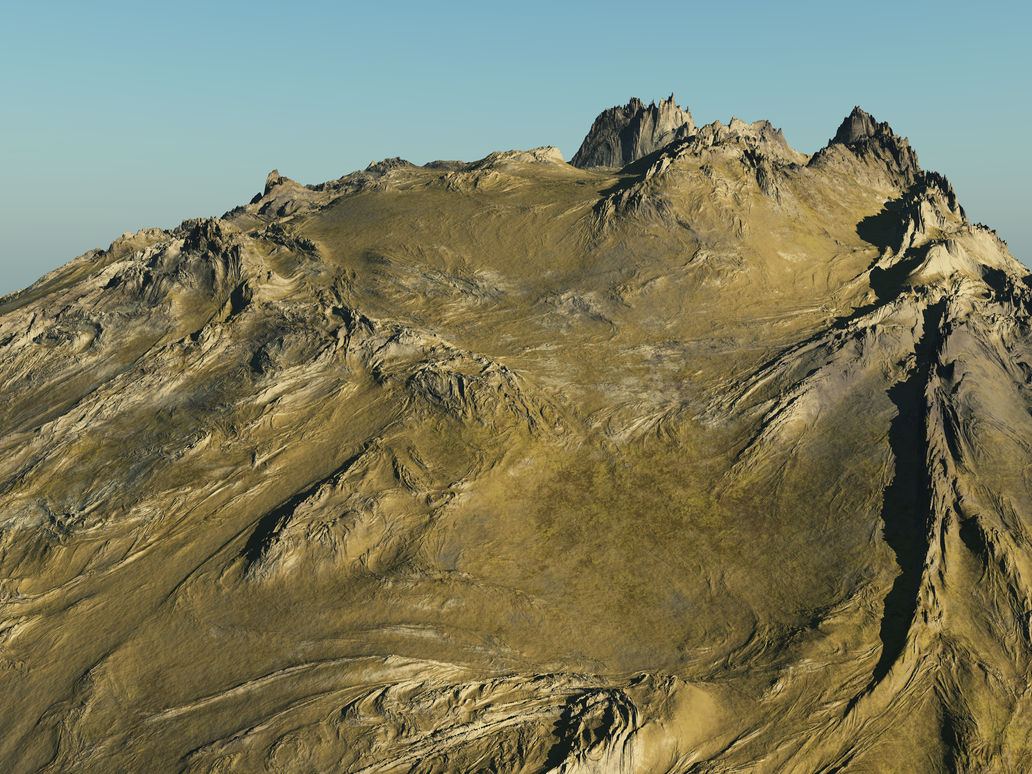
\includegraphics[width=0.4\textwidth]{images/terrain.png}
    \caption{Anwendung Perlin Noise}
\end{figure}
\end{frame}



\begin{frame}
    \frametitle{Algorithmen und Datenstrukturen}
\framesubtitle{}
\begin{block}{Perlin Noise}
Generiere Zufallsvektoren an Gitterpunkten.
\end{block}
\begin{figure}[H]
    \centering
    \includegraphics[width=0.8\textwidth]{images/perlinNoiseNV.png}
    \caption{Zufallsvektoren}
\end{figure}
\end{frame}

\begin{frame}
    \frametitle{Algorithmen und Datenstrukturen}
\framesubtitle{}
\begin{block}{Perlin Noise}
Berechne Skalarprodukte von Punkt mit Zufallsvektoren in zugehörigem 
Gittereckpunkten. Interpoliere zwischen diesen Werten. 
\end{block}
\begin{figure}[H]
    \centering
    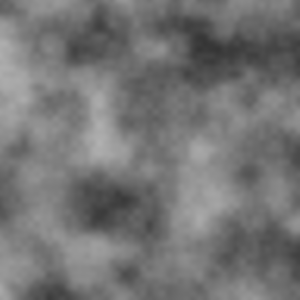
\includegraphics[width=0.4\textwidth]{images/perlin_noise.png}
    \caption{Perlin Noise Textur}
\end{figure}
\end{frame}


\begin{frame}
    \frametitle{Algorithmen und Datenstrukturen}
\framesubtitle{}
\begin{block}{Kd-Trees}
Kd-Trees sind balancierte Binärbäume, mit deren Hilfe Bereichsabfragen effizient
implementiert werden können.
\end{block}
\begin{figure}[H]
    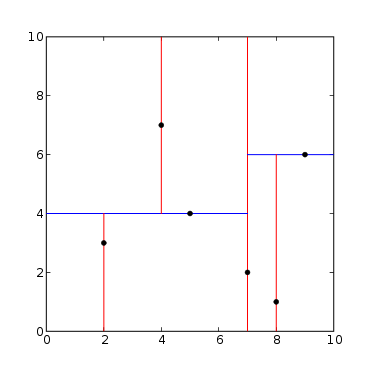
\includegraphics[width=0.4\textwidth]{images/kdtree_2d.png}
    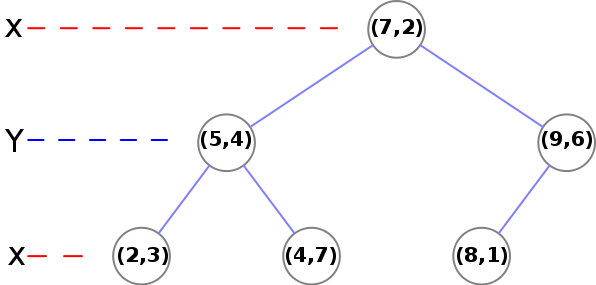
\includegraphics[width=0.4\textwidth]{images/kdtree.png}
\end{figure}
\end{frame}

\end{document}
